
%\documentclass[mathserif]{beamer}
\documentclass[handout]{beamer}
%\usetheme{Goettingen}
%\usetheme{Warsaw}
\usetheme{Singapore}



%\usetheme{Frankfurt}
%\usetheme{Copenhagen}
%\usetheme{Szeged}
%\usetheme{Montpellier}
%\usetheme{CambridgeUS}
%\usecolortheme{}
%\setbeamercovered{transparent}
\usepackage[english, activeacute]{babel}
\usepackage[utf8]{inputenc}
\usepackage{amsmath, amssymb}
\usepackage{dsfont}
\usepackage{graphics}
\usepackage{cases}
\usepackage{graphicx}
\usepackage{pgf}
\usepackage{epsfig}
\usepackage{amssymb}
\usepackage{multirow}	
\usepackage{amstext}
\usepackage[ruled,vlined,lined]{algorithm2e}
\usepackage{amsmath}
\usepackage{epic}
\usepackage{epsfig}
\usepackage{fontenc}
\usepackage{framed,color}
\usepackage{palatino, url, multicol}
%\algsetup{indent=2em}
\newcommand{\factorial}{\ensuremath{\mbox{\sc Factorial}}}
\newcommand{\BIGOP}[1]{\mathop{\mathchoice%
{\raise-0.22em\hbox{\huge $#1$}}%
{\raise-0.05em\hbox{\Large $#1$}}{\hbox{\large $#1$}}{#1}}}
\newcommand{\bigtimes}{\BIGOP{\times}}
\vspace{-0.5cm}
\title{Natural Language Processing \\ Recurrent Neural Networks}
\vspace{-0.5cm}
\author[Felipe Bravo Márquez]{\footnotesize
%\author{\footnotesize  
 \textcolor[rgb]{0.00,0.00,1.00}{Felipe Bravo-Marquez}} 
  
 

\date{\today}

\begin{document}
\begin{frame}
\titlepage


\end{frame}




\begin{frame}{Recurrent Neural Networks}
\begin{scriptsize}
\begin{itemize}

\item While representations derived from convolutional networks  offer some sensitivity to word order, their order sensitivity is restricted to mostly local patterns, and disregards the order of patterns that are far apart in the sequence.
\item Recurrent neural networks (RNNs) allow representing arbitrarily sized sequential inputs in fixed-size vectors, while paying attention to the structured properties of the inputs \cite{goldberg2016primer}.
\item RNNs, particularly ones with gated architectures such as the LSTM and the GRU, are very powerful at capturing statistical regularities in sequential inputs.

\end{itemize}
\end{scriptsize}
\end{frame}


\begin{frame}{The RNN Abstraction}
\begin{scriptsize}
\begin{itemize}

\item We use $\vec{x}_{i:j}$ to denote the sequence of vectors $\vec{x}_i, \dots, \vec{x}_j$.

\item On a high-level, the RNN is a function that takes as input an arbitrary length ordered sequence of $n$ $d_{in}$-dimensional vectors $\vec{x}_{i:n}=\vec{x}_1,\vec{x}_2, \dots, \vec{x}_n$ ( $\vec{x}_i \in  \mathcal{R}^{d_{in}}$) and returns as output a single $d_{out}$ dimensional vector $\vec{y}_n$ $\in \mathcal{R}^{d_{out}}$:

\begin{equation}
\begin{split}
\vec{y}_n & = RNN(\vec{x}_{1:n}) \\
\vec{x}_i \in  \mathcal{R}^{d_{in}} & \quad  \vec{y}_n  \in \mathcal{R}^{d_{out}}
\end{split}
\end{equation}

\item This implicitly defines an output vector $\vec{y}_i$ for each prefix $\vec{x}_{1:i}$ of the sequence $\vec{x}_{i:n}$.
\item We denote by $RNN^{*}$ the function returning this sequence:
\begin{equation}
\begin{split}
\vec{y}_{1:n} & = RNN^{*}(\vec{x}_{1:n}) \\
\vec{y}_i & = RNN(\vec{x}_{1:i}) \\
\vec{x}_i \in  \mathcal{R}^{d_{in}} & \quad  \vec{y}_n  \in \mathcal{R}^{d_{out}}
\end{split}
\end{equation}

\end{itemize}
\end{scriptsize}
\end{frame}


\begin{frame}{The RNN Abstraction}
\begin{scriptsize}
\begin{itemize}

\item The output vector $\vec{y}_n$ is then used for further prediction.
\item For example, a model for predicting the conditional probability of an event $e$ given the sequence $\vec{x}_{1:n}$ can be defined as the $j$-th element in the output vector resulting from the softmax operation over a linear transformation of the RNN encoding:
\begin{displaymath}
p(e = j|\vec{x}_{1:n}) = \text{softmax}(RNN(\vec{x}_{1:n})\cdot W +b)_{[j]} 
\end{displaymath}
\item The RNN function provides a framework for conditioning on the entire history without resorting to the Markov assumption which is traditionally used for modeling sequences.
\end{itemize}
\end{scriptsize}
\end{frame}



\begin{frame}{The RNN Abstraction}
\begin{scriptsize}
\begin{itemize}
\item The RNN is defined recursively, by means of a function $R$ taking as input a state vector $\vec{s}_{i-1}$  and an input vector $\vec{x}_{i}$ and returning a new state vector $\vec{s}_i$. 
\item The state vector $\vec{s}_i$ is then mapped to an output vector $\vec{y}_i$ using a simple deterministic function $O(\cdot)$.
\item The base of the recursion is an initial state vector, $\vec{s}_{0}$ , which is also an input to the RNN.
\item For brevity, we often omit the initial vector $s_{0}$ , or assume it is the zero vector.
\item When constructing an RNN, much like when constructing a feed-forward network, one has to specify the dimension of the inputs $\vec{x}_i$ as well as the dimensions of the outputs $\vec{y}_i$. 
\end{itemize}
\end{scriptsize}
\end{frame}




\begin{frame}{The RNN Abstraction}
\begin{scriptsize}

\begin{equation}
\begin{split}
 RNN^{*}(\vec{x}_{1:n};\vec{s}_0) & = \vec{y}_{1:n} \\
\vec{y}_i & = O(\vec{s}_i) \\
\vec{s}_i & = R(\vec{s}_{i-1},\vec{x}_i) \\
\vec{x}_i \in \mathcal{R}^{d_{in}}, & \quad \vec{y}_i \in \mathcal{R}^{d_{out}}, \quad \vec{s}_i \in \mathcal{R}^{f(d_{out})}
\end{split}
\end{equation}
\begin{itemize}
\item The functions $R$ and $O$ are the same across the sequence positions. 
\item The RNN keeps track of the states of computation through the state vector $\vec{s}_i$ that is kept and being passed across invocations of $R$.


\end{itemize}
\end{scriptsize}
\end{frame}




\begin{frame}{The RNN Abstraction}
\begin{scriptsize}

  \begin{figure}[h]
        	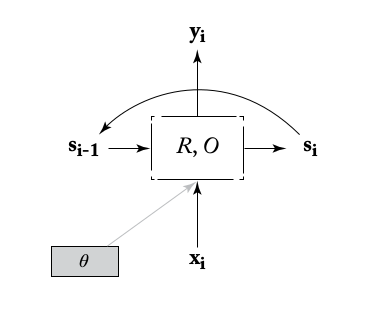
\includegraphics[scale = 0.4]{pics/RNN.png}
        \end{figure}
\begin{itemize}
\item This presentation follows the recursive definition, and is correct for arbitrarily long sequences.
\end{itemize}
\end{scriptsize}
\end{frame}




\begin{frame}{The RNN Abstraction}
\begin{scriptsize}
\begin{itemize}
\item For a finite sized input sequence (and all input sequences we deal with are finite) one can unroll the recursion.
  \begin{figure}[h]
        	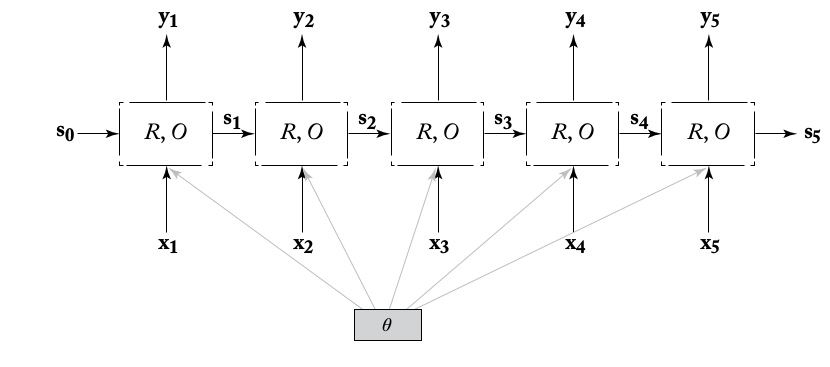
\includegraphics[scale = 0.35]{pics/RNN-unrolled.png}
        \end{figure}

        
\item The parameters $\theta$ highlight the fact that the same parameters are shared across all time steps. 
\item Different instantiations of $R$ and $O$ will result in different network structures.
\end{itemize}
\end{scriptsize}
\end{frame}


\begin{frame}{The RNN Abstraction}
\begin{scriptsize}
\begin{itemize}
\item We note that the value of $\vec{s}_i$  (and hence $\vec{y}_i$) is based on the entire input $\vec{x}_1,\dots, \vec{x}_i$.
\item For example, by expanding the recursion for $i = 4$ we get:
  \begin{figure}[h]
        	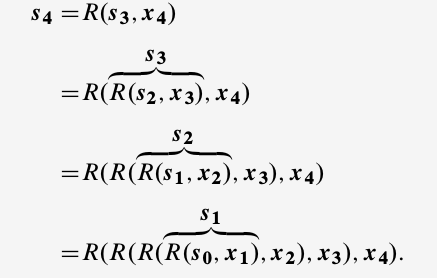
\includegraphics[scale = 0.35]{pics/RNN-recursion.png}
        \end{figure}
\item Thus, $\vec{s}_n$ and $\vec{y}_n$ can be thought of as encoding the entire input sequence.
\item The job of the network training is to set the parameters of $R$ and $O$ such that the state conveys useful information for the task we are tying to solve.

\end{itemize}
\end{scriptsize}
\end{frame}


\begin{frame}{RNN Training}
\begin{scriptsize}
\begin{itemize}
\item An unrolled RNN is just a very deep neural network.
\item The same parameters are shared across many parts of the computation.
\item Additional input is added at various layers.
\item To train an RNN network, need to create the unrolled computation graph for a given input sequence, add a loss node to the unrolled graph.
\item Then use the backward (backpropagation) algorithm to compute the gradients with respect to that loss.
\end{itemize}
\end{scriptsize}
\end{frame}

\begin{frame}{RNN Training}
\begin{scriptsize}
\begin{itemize}
\item This procedure is referred to in the RNN literature as backpropagation through time (BPTT).
\item The RNN does not do much on its own, but serves as a trainable component in a larger network.
\item The final prediction and loss computation are performed by that larger network, and the error is back-propagated through the RNN.
\item This way, the RNN learns to encode properties of the input sequences that are
useful for the further prediction task.
\item The supervision signal is not applied to the RNN directly, but through the larger network.
\end{itemize}
\end{scriptsize}
\end{frame}





\begin{frame}{Bidirectional RNNS (BIRNN)}
\begin{scriptsize}
\begin{itemize}
\item A useful elaboration of an RNN is a bidirectional-RNN (also commonly referred to as biRNN)
\item Consider the task of sequence tagging over a sentence.
\item An RNN allows us to compute a function of the $i$-th word $x_i$ based on the
past words $x_{1:i}$ up to and including it. 
\item However, the following words $x_{i+1:n}$ may also be useful for prediction,
\item The biRNN allows us to look arbitrarily far at both the past and the future within the sequence.
\end{itemize}
\end{scriptsize}
\end{frame}



\begin{frame}{Bidirectional RNNS (BIRNN)}
\begin{scriptsize}
\begin{itemize}
\item Consider an input sequence $\vec{x}_{1:n}$ . 
\item The biRNN works by maintaining two separate states, $s_{i}^{f}$ and $s_{i}^{b}$ for each input position $i$. 
\item The forward state $s_{i}^{f}$ is based on $\vec{x}_1, \vec{x}_2, \dots ,\vec{x}_i$, while the backward state $s_{i}^{b}$ is based on $\vec{x}_n, \vec{x}_{n-1}, \dots ,\vec{x}_i$.
\item The forward and backward states are generated
by two different RNNs.
\item The first RNN$(R^f, O^f)$  is fed the input sequence  $\vec{x}_{1:n}$ as is, while the second RNN$(R^b , O^b)$ is fed the input sequence in reverse.
\item The state representation $\vec{s}_i$ is then composed of both the forward and backward states.
\end{itemize}
\end{scriptsize}
\end{frame}


\begin{frame}{Bidirectional RNNS (BIRNN)}
\begin{scriptsize}
\begin{itemize}
\item The output at position $i$ is based on the concatenation of the two output vectors:
\begin{displaymath}
\vec{y}_i = [\vec{y}_{i}^{f};\vec{y}_{i}^{b}]=[O^{f}(s_{i}^{f});O^{b}(s_{i}^{b})
]
\end{displaymath}
\item The output takes into account both the past and the future.
\item The biRNN encoding of the $i$th word in a sequence is the concatenation of two RNNs, one reading the sequence from the beginning, and the other reading it from the end.
\item We define $biRNN(\vec{x}_{1:n}, i)$ to be the output vector corresponding to the $i$th sequence position:
\begin{displaymath}
biRNN(\vec{x}_{1:n}, i) = \vec{y}_i = [RNN^{f}(\vec{x}_{1:i});RNN^{b}(\vec{x}_{n:i})
\end{displaymath}
\end{itemize}
\end{scriptsize}
\end{frame}


\begin{frame}{Bidirectional RNNS (BIRNN)}
\begin{scriptsize}
\begin{itemize}
\item The vector $\vec{y}_i$ can then be used directly for prediction, or fed as part of the input to a more complex network.
\item While the two RNNs are run independently of each other, the error gradients
at position i will flow both forward and backward through the two RNNs.
\item Feeding the vector $\vec{y}_i$ through an MLP prior to prediction will further mix the forward and backward signals.
  \begin{figure}[h]
        	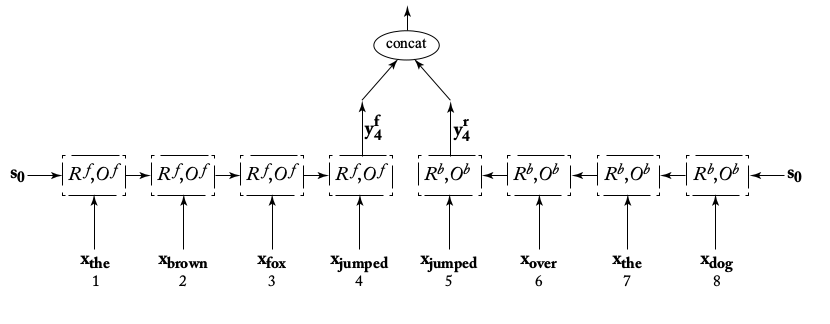
\includegraphics[scale = 0.35]{pics/biRNN.png}
        \end{figure}

\item Note how the vector $\vec{y}_4$ , corresponding to the word \textbf{jumped}, encodes an infinite window around (and including) the focus vector $\vec{x}_{jumped}$.        
\end{itemize}
\end{scriptsize}
\end{frame}


\begin{frame}{Bidirectional RNNS (BIRNN)}
\begin{scriptsize}
\begin{itemize}
\item Similarly to the $RNN$ case, we also define $biRNN^{*}(\vec{x}_{1:n})$ as the sequence of vectors $\vec{y}_{1:n}$:    
\begin{displaymath}
biRNN^{*}(\vec{x}_{1:n})= \vec{y}_{1:n} = biRNN(\vec{x}_{1:n},1),\dots,biRNN(\vec{x}_{1:n},n)
\end{displaymath}
\item The $n$ output vectors $\vec{y}_{1:n}$ can be efficiently computed in linear time by first running the forward and backward RNNs, and then concatenating the relevant outputs.
\end{itemize}
\end{scriptsize}
\end{frame}


\begin{frame}{Bidirectional RNNS (BIRNN)}
\begin{scriptsize}

  \begin{figure}[h]
        	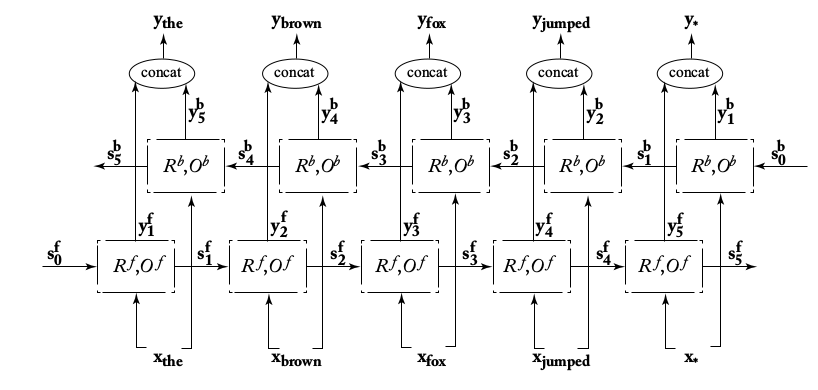
\includegraphics[scale = 0.35]{pics/biRNNstar.png}
        \end{figure}


\begin{itemize}

\item The biRNN is very effective for tagging tasks, in which each input vector corresponds to one output vector.

\item It is also useful as a general-purpose trainable feature-extracting component, that can be used whenever a window around a given word is required.
\end{itemize}
\end{scriptsize}
\end{frame}


\begin{frame}{Multi-layer (stacked) RNNS}
\begin{scriptsize}
\begin{itemize}
\item RNNs can be stacked in layers, forming a grid.
\item Consider $k$ RNNs, $RNN_{1},\dots, RNN_{k}$, where the $j$th RNN has states $\vec{s}_{1:n}^{j}$  and outputs $\vec{y}_{1:n}^{j}$.
\item The input for the first RNN are $\vec{x}_{1:n}$.
\item The input of the $j$th RNN ($j\geq 2$) are the outputs of the RNN below it, $\vec{y}_{1:n}^{j-1}$.
\item The output of the entire formation is the output of the last RNN, $\vec{y}_{1:n}^k$.
\item Such layered architectures are often called deep RNNs.
\end{itemize}
\end{scriptsize}
\end{frame}


\begin{frame}{Multi-layer (stacked) RNNS}
\begin{scriptsize}
  \begin{figure}[h]
        	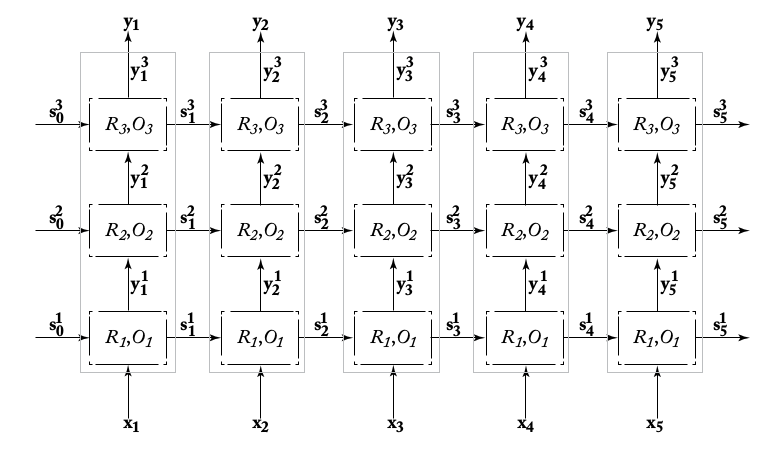
\includegraphics[scale = 0.35]{pics/stackedRNN.png}
        \end{figure}
\begin{itemize}
\item It is not theoretically clear what is the additional power gained by the deeper architecture.
\item It was observed empirically that deep RNNs work better than shallower ones on some tasks (e.g., machine translation).
\end{itemize}
\end{scriptsize}
\end{frame}


\begin{frame}{Elman Network or Simple-RNN}
\begin{scriptsize}
\begin{itemize}
\item After describing the RNN abstraction, we are now in place to discuss specific instantiations of it.
\item Recall that we are interested in a recursive function $\vec{s}_i =  R(\vec{x}_i, \vec{s}_{i-1})$ such that $\vec{s}_i$ encodes the sequence $\vec{x}_{1:n}$.
\item The simplest RNN formulation is known as an Elman Network or Simple-RNN (S-RNN).
\end{itemize}
\end{scriptsize}
\end{frame}

\begin{frame}{Elman Network or Simple-RNN}
\begin{scriptsize}
\begin{equation}
\begin{split}
\vec{s}_i & = R_{SRNN}(\vec{x}_{i},\vec{s}_{i-1}) = g(\vec{s}_{i-1}W^{s}+\vec{x}_{i}W^{x}+\vec{b}) \\
\vec{y}_i & = O_{SRNN}(\vec{s}_i) = \vec{s}_i \\
\vec{s}_i, \vec{y}_i \in  \mathcal{R}^{d_{s}}, & \quad  \vec{x}_i  \in \mathcal{R}^{d_{x}}, \quad W^{x} \in \mathcal{R}^{d_{x}\times d_{s}}, \quad W^{s} \in \mathcal{R}^{d_{s}\times d_{s}}, \vec{b} \in \mathcal{R}^{d_{s}} 
\end{split}
\end{equation}


\begin{itemize}
\item The state $\vec{s}_i$ and the input $\vec{x}_i$ are each linearly transformed.
\item The results are added (together with a bias term) and then passed through a nonlinear activation function g (commonly tanh or ReLU).
\item The Simple RNN provides strong results for sequence tagging as well as language modeling.
\end{itemize}
\end{scriptsize}
\end{frame}


\begin{frame}{Gated Architectures}
\begin{scriptsize}
\begin{itemize}
\item The S-RNN is hard to train effectively because of the \textbf{vanishing gradients} problem.
\item Error signals (gradients) in later steps in the sequence diminish quickly in the backpropagation process.
\item Thus, they do not reach earlier input signals, making it hard for the S-RNN to capture long-range dependencies.
\item Gating-based architectures, such as the LSTM [Hochreiter
and Schmidhuber, 1997] and the GRU [Cho et al., 2014b] are designed to solve this deficiency.
\end{itemize}
\end{scriptsize}
\end{frame}


\begin{frame}{Gated Architectures}
\begin{scriptsize}
\begin{itemize}
\item Consider the RNN as a general purpose computing device, where the state $\vec{s}_i$ represents a finite memory.
\item Each application of the function $R$ reads in an input $\vec{x}_{i+1}$ , reads in the current memory $\vec{s}_i$ , operates on them in some way, and writes the result into memory.
\item This resuls in a new memory state $\vec{s}_{i+1}$.
\item An apparent problem with the S-RNN architecture is that the memory access is not controlled. 
\item At each step of the computation, the entire memory state is read, and the entire memory state is written.
\end{itemize}
\end{scriptsize}
\end{frame}


\begin{frame}{Gated Architectures}
\begin{scriptsize}
\begin{itemize}
\item How does one provide more controlled memory access?
\item Consider a binary vector $\vec{g} \in {0,1}^n$. 
\item Such a vector can act as a \textbf{gate} for controlling access to $n$-dimensional vectors, using the hadamard-product operation $\vec{x} \odot \vec{g}$.
\item The hadamard operation is the same as the element-wise multiplication of two vectors:
\begin{displaymath}
\vec{x} = \vec{u} \odot \vec{v}  \Leftrightarrow  \vec{x}_{[i]} = \vec{u}_{[i]} \cdot \vec{v}_{[i]} \quad \forall i \in [1,n]
\end{displaymath}
\end{itemize}
\end{scriptsize}
\end{frame}




\begin{frame}{Gated Architectures}
\begin{scriptsize}
\begin{itemize}
\item Consider a memory $\vec{s} \in \mathcal{R}^{d}$, an input $\vec{x} \in \mathcal{R}^{d}$ and a gate $\vec{g} \in [0,1]^{d}$.
\item The following computation:
\begin{displaymath}
\vec{s}' \leftarrow \vec{g} \odot \vec{x} + (\vec{1}-\vec{g}) \odot (\vec{s}) 
\end{displaymath}
\item Reads the entries in $\vec{x}$ that correspond to the $\vec{1}$ values in $\vec{g}$ , and writes them to the new memory $\vec{s}'$.
\item Locations that weren't read to are copied from the memory $\vec{s}$ to the new memory $\vec{s}'$ through the use of the gate $(\vec{1}-\vec{g})$.
\end{itemize}
\end{scriptsize}
\end{frame}



\begin{frame}{Gated Architectures}
\begin{scriptsize}
  \begin{figure}[h]
        	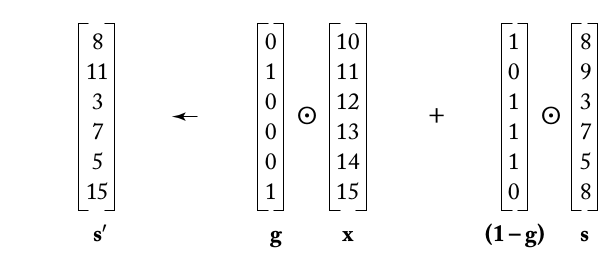
\includegraphics[scale = 0.35]{pics/gatedEx.png}
        \end{figure}
\begin{itemize}
\item This gating mechanism can serve as a building block in our RNN.
\item Gate vectors can be used to control access to the memory state $\vec{s}_i$.
\item We are still missing two important (and related) components: 
\begin{enumerate}
\begin{scriptsize}
 \item The gates should not be static, but be controlled by the
current memory state and the input.
\item Their behavior should be learned.
\end{scriptsize} 
\end{enumerate}
\item This introduced an obstacle, as learning in our framework entails being differentiable (because of the backpropagation algorithm).
\item The binary 0-1 values used in the gates are not differentiable.
\end{itemize}
\end{scriptsize}
\end{frame}


\begin{frame}{Gated Architectures}
\begin{scriptsize}

\begin{itemize}
\item A solution to this problem is to approximate the hard gating mechanism with a soft—but differentiable—gating mechanism.
\item To achieve these differentiable gates , we replace the requirement that $\vec{g} \in {0,1}^n$ and allow arbitrary real numbers, $\vec{g}' \in \mathcal{R}^n$.
\item These real numbers are then pass through a sigmoid function $\sigma(\vec{g}')$.
\item This bounds the value in the range $(0,1)$, with most values
near the borders.
\end{itemize}
\end{scriptsize}
\end{frame}



\begin{frame}{Gated Architectures}
\begin{scriptsize}

\begin{itemize}
\item When using the gate $\sigma(g')\odot \vec{x}$ , indices in $\vec{x}$ corresponding to near-one values in $\sigma(\vec{g}')$ are allowed to pass.
\item While those corresponding to near-zero values are blocked. 
\item The gate values can then be conditioned on the input and the current memory.
\item And can be trained using a gradient-based method to perform a desired behavior.
\item This controllable gating mechanism is the basis of the LSTM and the GRU architectures.
\item At each time step, differentiable gating mechanisms decide which parts of the inputs will be written to memory and which parts of memory will be overwritten (forgotten). 
\end{itemize}
\end{scriptsize}
\end{frame}


\begin{frame}{LSTM}
\begin{scriptsize}

\begin{itemize}
\item The Long Short-Term Memory (LSTM) architecture [Hochreiter and Schmidhuber, 1997] was designed to solve the vanishing gradients problem.
\item It was the the first architecture to introduce the gating mechanism.
\item The LSTM architecture explicitly splits the state vector $\vec{s}_i$ into two halves: 1) memory cells and 2) working memory.
\item The memory cells are designed to preserve the memory, and also the error gradients, across time, and are controlled through differentiable gating components\footnote{Smooth mathematical functions that simulate logical gates.}.
\item At each input state, a gate is used to decide how much of the new input should be written to the memory cell, and how much of the current content of the memory cell should be forgotten.
\end{itemize}
\end{scriptsize}
\end{frame}


\begin{frame}{LSTM}
\begin{scriptsize}

\begin{itemize}
\item Mathematically, the LSTM architecture is defined as:
  \begin{figure}[h]
        	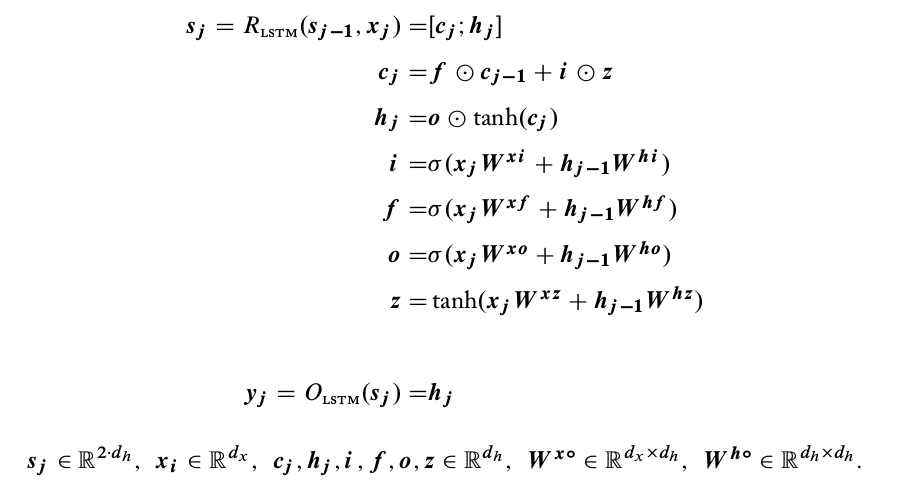
\includegraphics[scale = 0.35]{pics/LSTMform.png}
        \end{figure}
\end{itemize}
\end{scriptsize}
\end{frame}


\begin{frame}{LSTM}
\begin{scriptsize}

\begin{itemize}
\item The state at time $j$ is composed of two vectors, $\vec{c}_j$ and $h_{j}$, where $\vec{c}_j$ is the memory component and $\vec{h}_j$ is the hidden state component.
\item There are three gates, $\vec{i}$ , $\vec{f}$ , and $\vec{o}$, controlling for \textbf{i}nput, \textbf{f}orget, and \textbf{o}utput.
\item The gate values are computed based on linear combinations of the current input $\vec{x}_j$ and the previous state $\vec{h}_{j-1}$, passed through a sigmoid activation function.
\item An update candidate $\vec{z}$ is computed as a linear combination of $\vec{x}_j$ and $\vec{h}_{j-1}$ , passed through a tanh activation function (to push the values to be between -1 and 1).
\item The memory $\vec{c}_j$ is then updated: the forget gate controls how much of the previous memory to keep ($\vec{f} \odot \vec{c}_{j-1}$), and the input gate controls how much of the proposed update to keep ($\vec{i} \odot  \vec{z}$). 
\item Finally, the value of $\vec{h}_j$ (which is also the output $\vec{y}_j$ ) is determined based on the content of the memory $\vec{c}_j$ , passed through a tanh nonlinearity and controlled by the output gate. 
\item The gating mechanisms allow for gradients related to the memory part $\vec{c}_j$ to stay high across very long time ranges.
\end{itemize}
\end{scriptsize}
\end{frame}



\begin{frame}{LSTM}
  \begin{figure}[h]
        	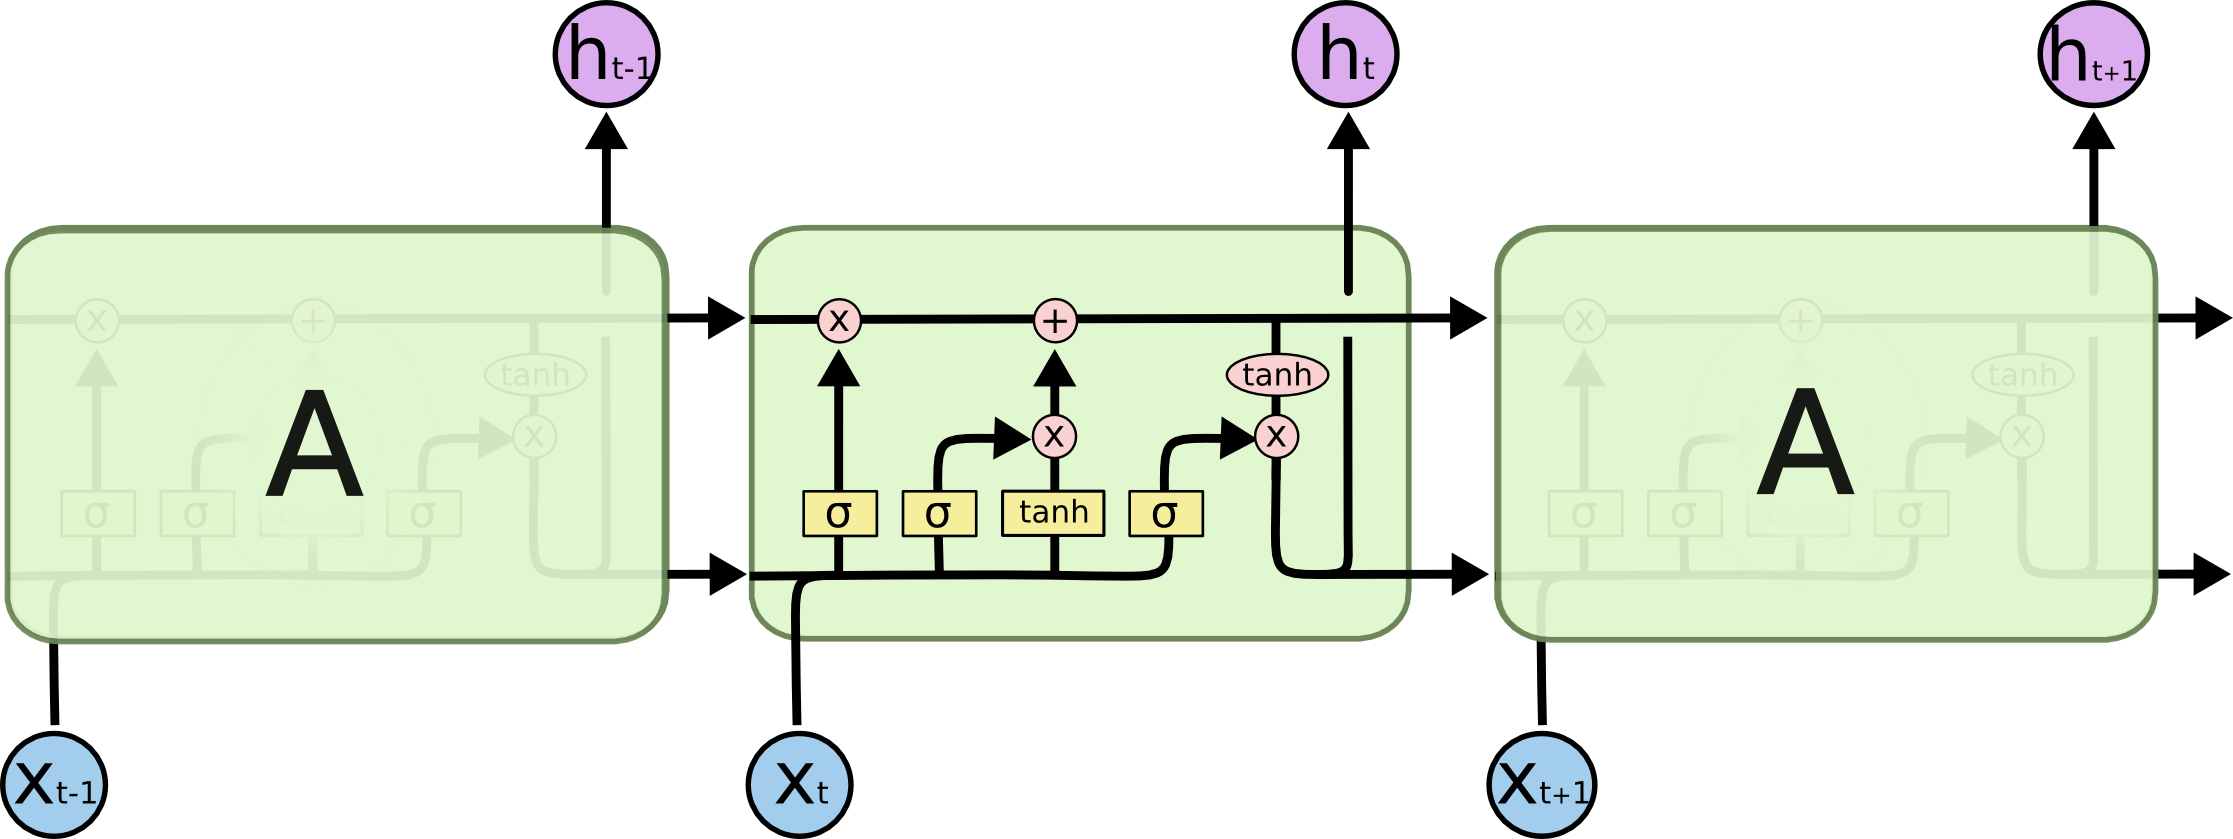
\includegraphics[scale = 0.35]{pics/LSTMchain.png}
        \end{figure}
\footnotemark{source: \url{http://colah.github.io/posts/2015-08-Understanding-LSTMs/}}        
\end{frame}


\begin{frame}{LSTM}
\begin{scriptsize}

\begin{itemize}
\item Intuitively, recurrent neural networks can be thought of as very deep feed-forward networks, with shared parameters across different layers.
\item For the Simple-RNN, the gradients then include repeated multiplication of the matrix $W$.
\item This makes the gradient values to vanish or explode.
\item The gating mechanism mitigate this problem to a large extent by getting rid of this repeated multiplication of a single matrix.
\item LSTMs are currently the most successful type of RNN architecture, and they are responsible for many state-of-the-art sequence modeling results.
\item The main competitor of the LSTM RNN is the GRU, to be discussed next.
\end{itemize}
\end{scriptsize}
\end{frame}



\begin{frame}{GRU}
\begin{scriptsize}

\begin{itemize}
\item The LSTM architecture is very effective, but also quite complicated.
\item The complexity of the system makes it hard to analyze, and also computationally expensive to work with.
\item The gated recurrent unit (GRU) was recently introduced by Cho et al. [2014b] as an alternative to the LSTM.
\item It was subsequently shown by Chung et al. [2014] to perform comparably to the LSTM on several (non textual) datasets.
\item Like the LSTM, the GRU is also based on a gating mechanism, but with substantially fewer gates and without a separate memory component.
\end{itemize}
\end{scriptsize}
\end{frame}



\begin{frame}{GRU}
  \begin{figure}[h]
        	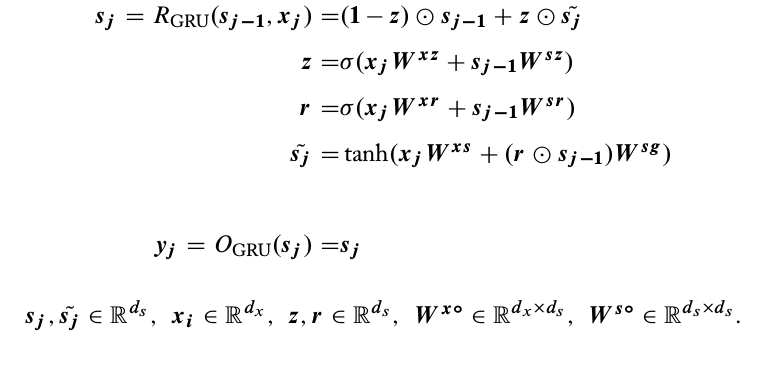
\includegraphics[scale = 0.35]{pics/GRU.png}
        \end{figure}        
\end{frame}



\begin{frame}{GRU}
\begin{scriptsize}
\begin{itemize}
\item One gate $\vec{r}$ is used to control access to the previous state $\vec{s}_{j-1}$ and compute a proposed update $\vec{\widetilde{s}}_j$.
\item The updated state $\vec{s}_j$ (which also serves as the output $\vec{y}_j$) is then determined based on an interpolation of the previous state $\vec{s}_{j-1}$ and the proposal $\vec{\widetilde{s}}_j$.
\item The proportions of the interpolation are controlled using the gate $\vec{z}$.
\item The GRU was shown to be effective in language modeling and machine translation.
\item However, the jury is still out between the GRU, the LSTM and possible alternative RNN architectures, and the subject is actively researched. 
\item For an empirical exploration of the GRU and the LSTM architectures, see Jozefowicz et al. [2015].
\end{itemize}
\end{scriptsize}
\end{frame}



\begin{frame}{Sentiment Classification with RNNs}
\begin{scriptsize}
\begin{itemize}
\item The simplest use of RNNs is as acceptors: read in an input sequence, and produce a binary or multi-class answer at the end.
\item RNNs are very strong sequence learners, and can pick-up on very
intricate patterns in the data.
\item An example of naturally occurring positive and negative sentences in the movie-reviews domain would be the following:
\item Positive: It's not life-affirming—it’s vulgar and mean, but I liked it.
\item Negative: It's a disappointing that it only manages to be decent instead of dead brilliant.
\end{itemize}
\end{scriptsize}
\end{frame}



\begin{frame}{Sentiment Classification with RNNs}
\begin{scriptsize}
\begin{itemize}
\item Note that the positive example contains some negative phrases (not life affirming, vulgar, and mean).
\item While the negative example contains some positive ones (dead brilliant).
\item Correctly predicting the sentiment requires understanding not only the individual phrases but also the context in which they occur, linguistic constructs such as negation, and the overall structure of the sentence.
\end{itemize}
\end{scriptsize}
\end{frame}

\begin{frame}{Sentiment Classification with RNNs}
\begin{scriptsize}
\begin{itemize}
\item The sentence-level sentiment classification task is modelled using an RNN-acceptor.
\item After tokenization, the RNN reads in the words of the sentence one at a time. \item The final RNN state is then fed into an MLP followed by a softmax-layer with two outputs (positive and negative). 
\item The network is trained with cross-entropy loss based on the gold sentiment labels.

\begin{equation}
\begin{split}
p(label = k | \vec{w}_{1:n}) & = \hat{\vec{y}}_{[k]} \\
\hat{\vec{y}} & = softmax(MLP(RNN(\vec{x}_{1:n}))) \\
\vec{x}_{1:n} & = E_{[w_{1}]}, \dots, E_{[w_{n}]} 
\end{split}
\end{equation}

\end{itemize}
\end{scriptsize}
\end{frame}




\begin{frame}{Sentiment Classification with RNNs}
\begin{scriptsize}
\begin{itemize}
\item The word embeddings matrix $E$ is initialized using pre-trained embeddings learned over a large external corpus using an algorithm such as word2vec or Glove with a relatively wide window.
\item It is often helpful to extend the model by considering bidirectional RNNs-
\item For longer sentences, Li et al. [2015] found it useful to use a hierarchical architecture, in which the sentence is split into smaller spans based on punctuation.
\item Then, each span is fed into a bidirectional RNN. 
\item Sequence of resulting vectors (onefor each span) are then fed into an RNN acceptor.
\item A similar hierarchical architecture was used for document-level sentiment classification in Tang et al. [2015].
\end{itemize}
\end{scriptsize}
\end{frame}

% https://arxiv.org/abs/1606.01781


\begin{frame}{Twitter Sentiment Classification with LSTMS Emojis}
\begin{scriptsize}
\begin{itemize}
\item An emoji-based distant supervision model for detecting sentiment and other affective states from short social media messages was proposed in \cite{FelboMSRL17}.
\item Emojis are used as a distant supervision approach for various affective detection tasks (e.g., emotion, sentiment, sarcasm) using a large corpus of 634M tweets with 64 emojis.
\item A neural network architecture is pretrained with this corpus. 
\item The network is an LSTM variant formed by an embedding layer, 2 bidrectional LSTM layers with normal skip connections and temporal average pooling-skip connections.
\end{itemize}
\end{scriptsize}
\end{frame}


\begin{frame}{DeepEmoji}
  \begin{figure}[h]
        	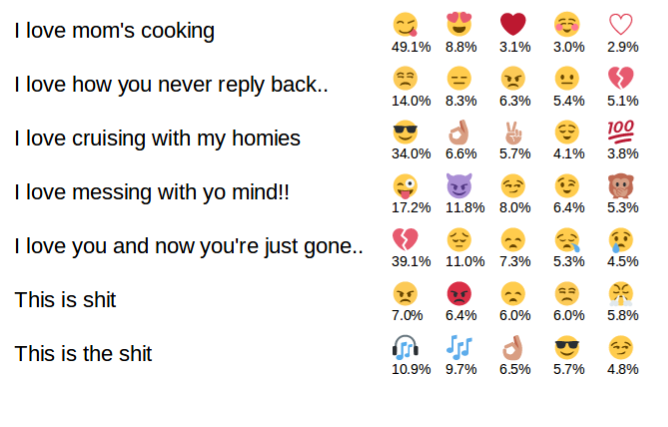
\includegraphics[scale = 0.45]{pics/deepEmoji1.png}
        \end{figure}    
        
\end{frame}




\begin{frame}{DeepEmoji}
   
    \begin{figure}[h]
        	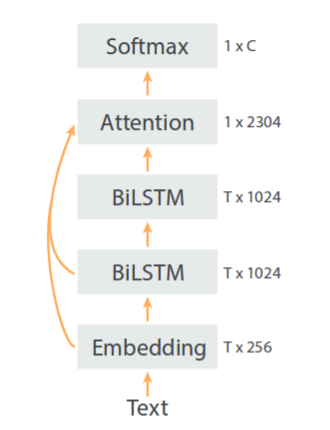
\includegraphics[scale = 0.45]{pics/deepEmoji2.png}
        \end{figure}       
        
\end{frame}




\begin{frame}{Twitter Sentiment Classification with LSTMS Emojis}
\begin{scriptsize}
\begin{itemize}
\item Authors propose the chain-thaw transfer-learning approach in which the pretrained network is fine-tuned for the target task. 
\item Here, each layer is individually fine-tuned in each step with the target gold data, and then they are all fine-tuned together. 
\item The model achieves state-of-the-art results the detection of emotion, sentiment, and sarcasm. 
\item  The pretrained network is released to the public.

\item  A demo of the model: \url{https://github.com/bfelbo/DeepMoji}.
\end{itemize}
\end{scriptsize}
\end{frame}


\begin{frame}{DeepEmoji}
        
         \begin{figure}[h]
        	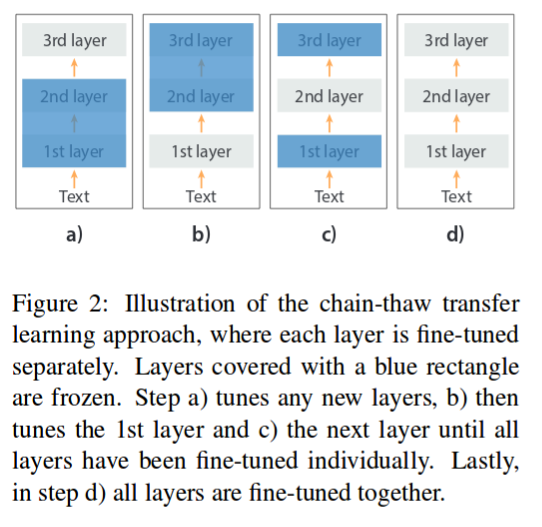
\includegraphics[scale = 0.45]{pics/deepEmoji3.png}
        \end{figure}        
        
\end{frame}





\begin{frame}
\frametitle{Questions?}
%\vspace{1.5cm}
\begin{center}\LARGE Thanks for your Attention!\\ \end{center}



\end{frame}

\begin{frame}[allowframebreaks]\scriptsize
\frametitle{References}
\bibliography{bio}
\bibliographystyle{apalike}
%\bibliographystyle{flexbib}
\end{frame}  


%%%%%%%%%%%%%%%%%%%%%%%%%%%

\end{document}
